\documentclass[UTF8]{ctexart}
\usepackage{amsmath}
\usepackage{graphicx}
\usepackage{float}
\usepackage{subfigure}
\usepackage{xeCJK}
\usepackage{hyperref}
\usepackage{algorithm2e}
\usepackage{amsfonts}
\usepackage{epsfig}
\usepackage{listings}
\usepackage{xcolor}
% 定义可能使用到的颜色

\definecolor{CPPLight}  {HTML} {686868}
\definecolor{CPPSteel}  {HTML} {888888}
\definecolor{CPPDark}   {HTML} {262626}
\definecolor{CPPBlue}   {HTML} {4172A3}
\definecolor{CPPGreen}  {HTML} {487818}
\definecolor{CPPBrown}  {HTML} {A07040}
\definecolor{CPPRed}    {HTML} {AD4D3A}
\definecolor{CPPViolet} {HTML} {7040A0}
\definecolor{CPPGray}  {HTML} {B8B8B8}
\lstset{
    columns=fixed,
    numbers=left,                                        % 在左侧显示行号
    frame=none,                                          % 不显示背景边框
    backgroundcolor=\color[RGB]{245,245,244},            % 设定背景颜色
    keywordstyle=\color[RGB]{40,40,255},                 % 设定关键字颜色
    numberstyle=\footnotesize\color{darkgray},           % 设定行号格式
    commentstyle=\it\color[RGB]{0,96,96},                % 设置代码注释的格式
    stringstyle=\rmfamily\slshape\color[RGB]{128,0,0},   % 设置字符串格式
    showstringspaces=false,                              % 不显示字符串中的空格
    language=c++,                                        % 设置语言
    morekeywords={alignas,continute,friend,register,true,alignof,decltype,goto,
    reinterpret_cast,try,asm,defult,if,return,typedef,auto,delete,inline,short,
    typeid,bool,do,int,signed,typename,break,double,long,sizeof,union,case,
    dynamic_cast,mutable,static,unsigned,catch,else,namespace,static_assert,using,
    char,enum,new,static_cast,virtual,char16_t,char32_t,explict,noexcept,struct,
    void,export,nullptr,switch,volatile,class,extern,operator,template,wchar_t,
    const,false,private,this,while,constexpr,float,protected,thread_local,
    const_cast,for,public,throw,std},
}

\graphicspath{{images/}}
\setCJKmonofont{Microsoft YaHei}

\title{\Huge{计算机算法设计与分析\\ 动态规划}}
\author{\Huge{易凯}}
\date{\Huge{2017年4月18日}}

\begin{document}
    \maketitle
    \vspace{35mm}
    \begin{flushright}
    \Large{
    \textbf{班\ \ \ \ \ 级} \makebox[5em][l]{软件53班}

    \textbf{学\ \ \ \ \ 号} \makebox[5em][l]{2151601053}

    \textbf{邮\ \ \ \ \ 箱} \makebox[5em][l]{williamyi96@gmail.com}

    \textbf{联系电话} \makebox[5em][l]{13772103675}

    \textbf{个人网站} \makebox[5em][l]{https://williamyi96.github.io}

                      \makebox[5em][l]{williamyi.tech}

      \textbf{实验日期} \makebox[5em][l]{2017年4月25日}

    \textbf{提交日期} \makebox[5em][l]{2017年6月6日}
    }
    \end{flushright}

    \newpage
  	\tableofcontents
  	\newpage
  	\listoffigures
    \newpage

    \section{贪心算法相关概念}
    贪心算法是一种逐步逼近最优解的算法,仅考虑当前如何决策可以达到最优,而不考虑全局最优。虽然由其得到的解不一定为最优解,但是其逼近最优解,或者说是最优解的一个近似解。

    \section{贪心算法基本要素}
    1. 贪心选择性质

    2. 最优子结构性质

    \section{贪心算法与动态规划的区别}
    贪心算法与动态规划的相同点是两者都需要研究的问题具有最优子结构。在动态规划算法中,每步所做的选择往往依赖于相关子问题的解,只有在解出相关子问题之后才能够做出选择;但是在贪心算法中,仅在当前状态下做出最好的选择,即局部最优选择。

    \section{哈夫曼编码问题}
    \subsection{试题描述}
    字符a-h出现的频率恰好是前8个Fibonacci数,它们的哈夫曼编码是什么?将结果推广到n个字符的频率恰好是前n个Fibonacci数的情形。

    \subsection{题目分析与求解}
    哈夫曼编码是一种将使用字符在文件中出现的频率表构建的不定长码。

    其中前八个Fibonacci数分别为1,1,2,3,5,8,13,21。

    \begin{figure}[!htb]
      \centering
      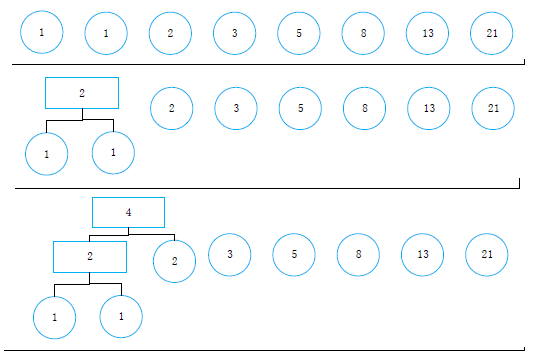
\includegraphics[width=0.6\textwidth]{../img/4.1.1.PNG}
      \caption{斐波那契哈夫曼编码1}\label{斐波那契哈夫曼编码1}
    \end{figure}

    \begin{figure}[!htb]
      \centering
      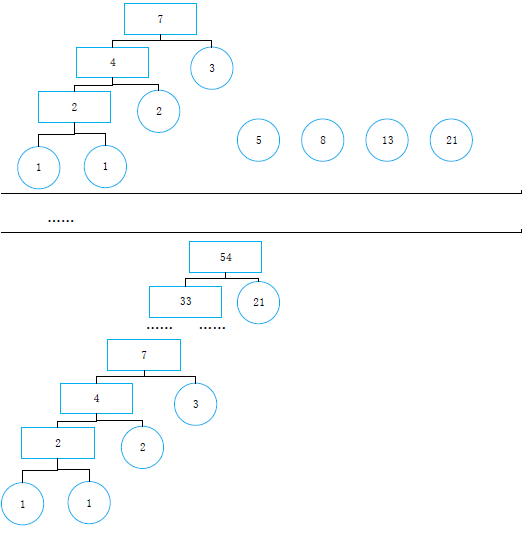
\includegraphics[width=0.6\textwidth]{../img/4.1.2.PNG}
      \caption{斐波那契哈夫曼编码2}\label{斐波那契哈夫曼编码2}
    \end{figure}

    如果是n个字符的频率满足Fibonacci数列的情况,则最终的结果为:

    \begin{figure}[!htb]
      \centering
      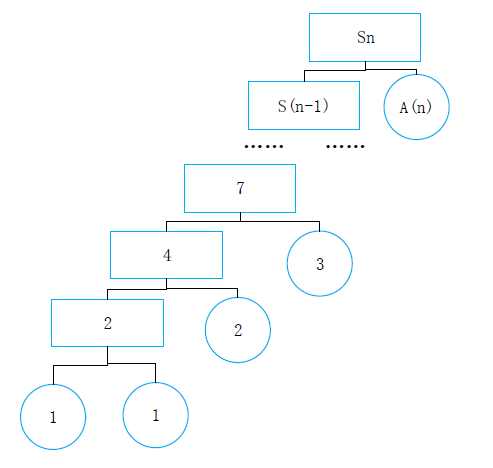
\includegraphics[width=0.6\textwidth]{../img/4.1.3.PNG}
      \caption{斐波那契哈夫曼编码3}\label{斐波那契哈夫曼编码3}
    \end{figure}

    \section{磁盘文件最优存储问题}
    \subsection{试题描述}
    设磁盘上有n个文件f1,f2,…,fn,每个文件占用磁盘上的1个磁道。这n个文件的检索概率分别是p1,p2,…,pn,且 =1。磁头从当前磁道移到被检信息磁道所需的时间可用这2个磁道之间的径向距离来度量。如果文件fi存放在第i道上,1≦i≦n,则检索这n个文件的期望时间是对于所有的i<j,time+=pi*pj*d(i,j) 。其中d(i,j)是第i道与第j道之间的径向距离|i-j|。
    磁盘文件的最优存储问题要求确定这n个文件在磁盘上的存储位置,使期望检索时间达到最小。
    \subsection{算法设计}
    对于戈丁的文件检索概率,计算磁盘文件的最优存储方案。
    \subsection{数据输入}
    第1行是正整数n,表示文件个数。第2行有n个正整数ai,表示文件的检索概率。
    \subsection{数据输出}
    计算的最小期望检索时间
    \subsection{问题分析}
    此题是使用贪心算法求解的典型,其中先将n个文件按访问概率从大到小进行排序,其中概率最大的放在中间磁道上,次大和次次大的放在最大的两边,逐级递推,最后访问概率最小的放在最边上。
    \subsection{程序代码}
    \begin{small}
    \begin{lstlisting}
#include <iostream>
#include <stdio.h>   
#include <algorithm>
using namespace std;   
  
int cmp (const void *a , const void *b) {    
    return *(double *)a - *(double *)b;    
}   
  
double greedy(double a[],int n) {   
    qsort(a,n,sizeof(double),cmp);   
    int mid = (n - 1) / 2;   
    double x[n];   
    x[mid] = a[n-1];   
    for(int i = mid+1;i < n;i++)   
        x[i] = a[n - 2*(i-mid)];   
    for(int i = mid-1;i >= 0;i--)   
        x[i] = a[n - 2*(mid-i) - 1];   
    double sum = 0,exp = 0;   
    for(int i = 0;i < n;i++) {   
        sum += a[i];   
        for(int j = i+1;j < n;j++)   
            exp += x[i]*x[j]*(j-i);   
    }   
    return exp/sum/sum;   
}   
           
int main() {   
    int i,j,n;   
    double a[1000],exp;   
    scanf("%d",&n);   
    for(i = 0;i < n;i++)   
        scanf("%lf",&a[i]);   
    exp = greedy(a,n);   
    printf("%lf\n",exp);    
} 
    \end{lstlisting}
    \end{small}
    \subsection{样例运行}
    \begin{figure}[!htb]
      \centering
      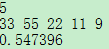
\includegraphics[width=0.3\textwidth]{../img/4.2.PNG}
      \caption{磁盘文件最优存储问题运行示例}\label{磁盘文件最优存储问题运行示例}
    \end{figure}
    
    \section{程序存储问题}
    \subsection{试题描述}
    设有n个程序{1,2,3...n}要存放在长度为L的磁带上,程序i存放在磁带上的长度为li。程序存储问题要求确定这n个程序在磁带上的一个存储方案,使得能够在磁带上存储尽可能多的程序。
    \subsection{算法设计}
    对于给定的n个程序存放在磁带上的长度,计算磁带上最多可以存储的程序数。
    \subsection{数据输入}
    输入的格式是第一行是两个正整数,分别表示文件个数n和磁带的长度l,接下来的一行中,有n个正整数,表示程序存放在磁盘上的长度。
    \subsection{数据输出}
    将计算的最多可以存储的程序数输出到文件中。
    \subsection{问题分析}
    此题可以使用贪心算法求解近似最优解。其满足贪心算法使用的贪心性质和最优子结构性质。因此其贪心策略就是将文件长度最小的文件存入磁带上。
    \subsection{程序代码}
    \begin{small}
    \begin{lstlisting}
#include<iostream>
#include<algorithm>
using namespace std;

int a[100000];

int most(int *a,int n,int s) {
  int i=0,sum=0;
  while(i<n) {
    sum=a[i]+sum;
    if(sum<=s) i++;
    else return i;
  }
  return n;
}

int main() {
  int i,n,s;
  scanf("%d %d\n",&n,&s);
  for(i=0;i<n;i++) scanf("%d",&a[i]);
  sort(a,a+n);
  printf("%d",most(a,n,s));
  return 0;
}
    \end{lstlisting}
    \end{small}
    \subsection{样例运行}
    \begin{figure}[!htb]
      \centering
      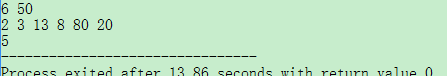
\includegraphics[width=1.0\textwidth]{../img/4.5.PNG}
      \caption{磁盘存储问题样例运行}\label{磁盘存储问题样例运行}
    \end{figure}

    \section{最优服务次序问题}
    \subsection{试题描述}
    设有n个顾客同时等待一项服务。顾客i需要的服务时间为ti,1<=i<=n。应该如何安排n个顾客的服务次序才能使平均等待时间达到最小?平均等待时间是n个顾客等待服务时间的总和除以n。
    \subsection{算法设计}
    对于给定的n个顾客需要的服务时间,计算最优服务次序。
    \subsection{数据输入}
    输入的格式中第一行为正整数n,表示n个顾客,接下来的一行中,有n个正整数,表示n个顾客需要的服务时间。
    \subsection{数据输出}
    计算出最小平均等待时间输出到屏幕之上。
    \subsection{问题分析}
    此题可以使用贪心算法来求得最优解。其中该题目具有贪心选择性质以及最优子结构性质。
    \subsection{程序代码}
    \begin{small}
    \begin{lstlisting}
#include<iostream>
#include<cstring>
#include<algorithm>
using namespace std;

int main()
{
  int n;
  cin >> n;
  int a[100] = { 0 };
  for (int i = 1; i <=n; i++)
    cin >> a[i];
  sort(a, a+n);
  double sum=0;
  for (int i = 1; i <= n; i++)
    sum +=(n+1-i)*a[i];
  cout << sum / n<<endl;
  return 0;
}
    \end{lstlisting}
    \end{small}
    \subsection{样例运行}
    \begin{figure}[!htb]
      \centering
      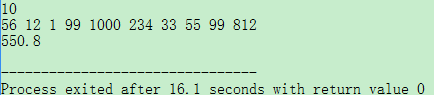
\includegraphics[width=0.6\textwidth]{../img/4.6.PNG}
      \caption{最优服务次序问题样例输出}\label{最优服务次序问题样例输出}
    \end{figure}

    \section{汽车加油问题}
    \subsection{试题描述}
    一辆汽车加满油后能够行驶nkm,旅途中有若干个加油站。设计一个有效的算法,指出应该在那些加油站停靠加油,使沿途加油次数最少,并证明算法能够产生一个最优解。
    \subsection{算法设计}
    对于给定的n和k个加油站位置,计算最少加油次数。
    \subsection{数据输入}
    文件的输入格式为第一行有两个正整数n和k,其中表示加满油可行驶nkm,且旅途中有k个加油站。接下来的一行中,有k+1个整数,表示第k个加油站与第k-1个加油站之间的距离。第0个加油站表示出发地,汽车已经加满了油。第k+1个加油站表示目的地。
    \subsection{数据输出}
    将计算的最少加油次数输出到屏幕上。如果无法叨叨目的地,则输出“No Solution”。
    \subsection{问题分析}

    \subsection{程序代码}
    \begin{small}
    \begin{lstlisting}
#include <stdio.h>   
  
void greedy(int d[],int n,int k) {   
    int num = 0;   
    for(int i = 0;i < k;i++) {   
        if(d[i] > n) {   
            printf("no solution/n");   
            return;   
        }   
    }   
    for(int i = 0,s = 0;i < k;i++) {   
        s += d[i];   
        if(s > n) {   
            num++;   
            s = d[i];   
        }   
    }   
    printf("%d\n",num);   
}   
             
int main() {   
    int i,n,k;   
    int d[1000];   
    scanf("%d %d",&n,&k);   
    for(i = 0;i < k;i++)   
        scanf("%d",&d[i]);   
    greedy(d,n,k);   
}  
    \end{lstlisting}
    \end{small}
    \subsection{样例运行}
    \begin{figure}[!htb]
      \centering
      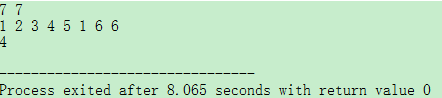
\includegraphics[width=1.0\textwidth]{../img/4.9.PNG}
      \caption{汽车加油问题样例运行}\label{汽车加油问题样例运行}
    \end{figure}
    \subsection{算法最优解证明}
    使用反证法。假设a为起始位点,b为终止位点,如果存在中间位点c使a-c加油次数更少,那么a-c,c-b联合所得到的加油次数最少,则原策略不是a-b的最优策略。但是可以使用a-c策略进行替换,使其具有最优策略。综上所述,算法能够产生最优解。\textbf{这么证明是否具有说服力??}

    \section{磁带最大利用率问题}
    \subsection{试题描述}
    设有n 个程序{1,2,…, n }要存放在长度为L的磁带上。程序i存放在磁带上的长度是li,1≤i≤n.程序存储问题要求确定这n个程序在磁带上的一个存储方案,使得能够在磁带上存储尽可能多的程序。在保证存储最多程序的前提下还要求磁带的利用率达到最大。
    \subsection{算法设计}
    对于给定的n个程序存放在磁带上的长度,编程计算磁带上最多可以存储的程序数和占用磁带的长度。
    \subsection{数据输入}
    第一行是2 个正整数,分别表示文件个数n和磁带的长度L。接下来的1 行中,有n个正整数,表示程序存放在磁带上的长度。
    \subsection{数据输出}
    第1 行输出最多可以存储的程序数和占用磁带的长度;第2行输出存放在磁带上的每个程序的长度。
    \subsection{程序代码}
    此题暂时没有找到一种好的贪心方式进行求解。
    
    \section{最优分解问题}
    \subsection{试题描述}
    设n是一个正整数。现在要求将n分解成若干个互不相同的自然数的和,且使这些自然数的乘积最大。
    \subsection{算法设计}
    对于给定的正整数n,计算最优分解方案。
    \subsection{数据输入}
    输入仅有一行,表示的是待分解的自然数。
    \subsection{数据输出}
    输出是计算得到的最大乘积。
    \subsection{问题分析}
    对整数分析可有结论:若a+b=const, 则|a–b|越小,a*b越大。根据原问题的描述,需要将正整数n分解为若干互不相同的自然数的和,同时又要使自然数的乘积最大。当n<4时,对n的分解的乘积是小于n的;当n大于或等于4时,n=1+(n–1)因的乘积也是小于n的,所以n=a+(n–a),2≤a≤n-2,可以保证乘积大于n,即越分解乘积越大。因此可以采用如下贪心策略:将n分成从2开始的连续自然数的和,如果最后剩下一个数将此数在后项优先的⽅式下均匀地分给前面各项。该贪心策略首先保证了正整数所分解出的因子之差的绝对值最小,即|a–b|最小;同时又可以将其分解成尽可能多的因子,且因子的值较大,确保最终所分解的自然数的乘积可以取得最大值。
    \subsection{程序代码}
    \begin{small}
    \begin{lstlisting}
#include<iostream>
using namespace std;
int main() {
    int n,sum=0,i,d;
    cin>>n;
    for(i=2;;++i) {
        sum+=i;
        d=sum-n;
        if(d>=0) break;
    }
    unsigned int result=1;
    if(d==1) {
        for(int j=3;j<i;++j) result*=j;
        i++;
        result *= i;
    } else {
        for(int j=2;j<=i;++j) {
            if(j==d) continue;
            result*=j;
        }
    }
    //cout<<"The result is "<<result<<endl;
    cout << result << endl;
    return 0;
}
    \end{lstlisting}
    \end{small}
    \subsection{样例运行}
    \begin{figure}[!htb]
      \centering
      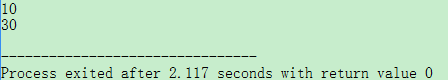
\includegraphics[width=0.6\textwidth]{../img/4.15.PNG}
      \caption{最优分解问题样例运行}\label{最优分解问题样例运行}
    \end{figure}
\end{document} 